\section{The SkelCL Library}
\label{section:skelcl-library}
In this section we discuss the \SkelCL Library -- our implementation of the \SkelCL programming model.
It provides a \Cpp~\API that implements the features of the \SkelCL programming model, and thus liberates the application developer from writing low-level code.
In addition, the library provides some commonly used utility functions, \eg, for program initialization.
The \SkelCL Library is open source software and available at: \url{http://skelcl.uni-muenster.de}.

We start our discussion with an example showing how to use the \SkelCL library.
We describe the syntax used to represent the \SkelCL programming model introduced in the previous section.
This will include a discussion of \Cpp techniques used to implement the library.
We then shift the focus to the implementations of the memory management, algorithmic skeletons, and distributions.










\subsection{Programming with the \SkelCL Library}

\autoref{lst:skelcl:dotproduct} shows the implementation of the dot product computation, discussed in the previous section, in \SkelCL.
After including the appropriate \SkelCL headers (\autoref{lst:skelcl:dotproduct:inc:start}---\autoref{lst:skelcl:dotproduct:inc:end}) the \SkelCL library can be initialized as shown in \autoref{lst:skelcl:dotproduct:init}.
This will perform the initializations required by \OpenCL.
The argument provided to the \code{init} function specifies how many and which \OpenCL devices should be used by \SkelCL.
Here a single device should be used which can be of any type, \ie, it can be either a \CPU or a \GPU.
The dot product is specified using the \zip and \reduce skeletons.
The skeletons are created using \code{zip} (\autoref{lst:skelcl:dotproduct:zip}) and \code{reduce} (\autoref{lst:skelcl:dotproduct:reduce}) functions which expect the customizing functions of the skeletons as arguments.
In this example we use \Cpp lambda expressions (\autoref{lst:skelcl:dotproduct:zip:lambda} and \autoref{lst:skelcl:dotproduct:reduce:lambda}) to specify the customizing functions of the skeletons.
We create the two input \code{Vector}s from C style pointers (\autoref{lst:skelcl:dotproduct:vecAB}).
In \autoref{lst:skelcl:dotproduct:apply} we perform the computation by applying the customized skeletons to the data, before we finally return the computed result in \autoref{lst:skelcl:dotproduct:return}.

\begin{lstlisting}[%
caption={Implementation of the dot product computation in \SkelCL.},%
float=t,%
numbers=left,%
label={lst:skelcl:dotproduct}]
#include <SkelCL/SkelCL.h>$\label{lst:skelcl:dotproduct:inc:start}$
#include <SkelCL/Zip.h>
#include <SkelCL/Reduce.h>
#include <SkelCL/Vector.h>$\label{lst:skelcl:dotproduct:inc:end}$

float dotProduct(const float* a, const float* b, int n) {
  using namespace skelcl;
  skelcl::init( 1_device.type(deviceType::ANY) );$\label{lst:skelcl:dotproduct:init}$

  auto mult = zip([](float x, float y) { return x*y; });$\label{lst:skelcl:dotproduct:zip}$$\label{lst:skelcl:dotproduct:zip:lambda}$
  auto sum = reduce([](float x, float y){ return x+y; }, 0);$\label{lst:skelcl:dotproduct:reduce}$$\label{lst:skelcl:dotproduct:reduce:lambda}$

  Vector<float> A(a, a+n); Vector<float> B(b, b+n);$\label{lst:skelcl:dotproduct:vecAB}$

  Vector<float> C = sum( mult(A, B) );$\label{lst:skelcl:dotproduct:apply}$

  return C.front();$\label{lst:skelcl:dotproduct:return}$
}
\end{lstlisting}

\autoref{lst:skelcl:dotproduct} shows that the \SkelCL library integrates nicely with \Cpp:
the interface of the \code{Vector} class looks familiar to \Cpp programmers and the usage of modern \Cpp features like lambda expressions, type deduction (\code{auto}), and user-defined literals simplify the programming as functions can be defined directly inline, type information can be omitted, and the specification of which devices to use can be written intuitively.

We will now discuss how our implementation enables this comfortable level of integrating \SkelCL with \Cpp.










\subsection{Syntax and Integration with \Cpp}
\label{section:skelcl-library:syntax}

The \SkelCL library is built on top of \OpenCL.
This offers clear benefits as well as introduces technical challenges.
One of the technical challenges is, that \OpenCL requires the kernel to be specified as a string in the host program.
While this enables portability across different hardware architectures, it also introduces a burden on the application developer as strong typing cannot be guaranteed statically when the host program is compiled.
For the implementation of \SkelCL, we choose to address this issue using a two-step implementation.
In the first step, a custom compiler transforms the source code as seen in \autoref{lst:skelcl:dotproduct} to a representation where the kernel computations are represented as strings as required by \OpenCL.
In the second step, the transformed program is compiled using a traditional \Cpp compiler to produce the final executable.

This allows ourselves to free the users from writing strings in their application code and maintain the usual type safety guarantees from \Cpp at compile time.
Furthermore, we implemented type inference capabilities in our source-to-source compiler to free the application developer from specifying type information explicitly.
Our two-step design also allows application developers to compile their application code into a form which then can be deployed on systems where it might be difficult to install a custom compiler.

In the next paragraph, we will start the discussion of our source-to-source compiler.
We will discuss how our custom compiler, together with our template-based implementation, helps to maintain strong type safety at compile time.
Finally, we will look at issues regarding the integration with \Cpp like sharing code between host and device code.

\paragraph{The custom SkelCL compiler}
To allow a deep integration of \SkelCL code with \Cpp, we implemented a custom compiler: \code{skelclc}.
We leverage the LLVM infrastructure~\cite{Lattner2004} for building this compiler.
LLVM and the related Clang project offer well-defined application programming interfaces for writing C and \Cpp related compiler tools.
In particular the \emph{LibTooling} API allows for writing tools which search for particular patterns in the abstract syntax tree (AST) which is representing the source code and perform actions on the found code fragments.
The \code{skelclc} custom compiler does exactly this.
For example, the custom compiler searches for an expression like this:
\begin{lstlisting}[numbers=none,label={lst:skelclc:before},caption={\SkelCL code snippet before transformation.}]
auto mult = zip( [](float x, float y){ return x*y; } );
\end{lstlisting}
and replaces it with:
\smallskip
\begin{lstlisting}[numbers=none,label={lst:skelclc:after},caption={\SkelCL code snippet after transformation.}]
auto mult = Zip<Container<float>(Container<float>,
                                 Container<float>)>(
              Source("float func(float x, float y)"
                     " { return x*y; }"), "func");
\end{lstlisting}

In this example, the \code{zip} function has been transformed into a call of the constructor of the \code{Zip} class and the lambda expression has been transformed into a string.
Furthermore, type information that has been inferred from the lambda expression, has been added to the templated \code{Zip} class.

The user is free to write the expression in \autoref{lst:skelclc:after} explicitly, but it is arguably more convenient to write the expression as in \autoref{lst:skelclc:before} and let \code{skelclc} perform the transformation automatically.

For every skeleton available in \SkelCL, there exists a function like \code{zip} which is transformed by \code{skelclc} to a call of the constructor of the corresponding skeleton class.

\paragraph{Maintaining type safety}
Each skeleton is represented by a templated class, as seen in \autoref{lst:skelclc:after} for the \zip skeleton.
The template arguments of the skeleton define the types which can be used when executing the skeleton.
For a skeleton of type \code{skeleton<T(U)>}, an object of type \code{U} has to be provided on execution to receive an object of type \code{T}.
In this respect skeletons behave exactly like functions in \Cpp which can be represented using the \code{std::function<T(U)>} template class.
Skeletons taking more then one argument (like the \code{zip} skeleton) are represented as \code{skeleton<T(U, V)>}.% using the \emph{variadic template} feature of \Cpp.

When performing the transformations, \code{skelclc} infers the types used as template arguments of the skeleton class.
To do so, it determines the types of the lambda expression arguments and skeleton's result type.
For \autoref{lst:skelclc:before} this is: \code{float} and \code{float} as argument types and \code{float} as the result type.
The result type is inferred following standard \Cpp rules.
Based on these types, the template arguments of the skeleton are constructed.

The skeletons \map, \zip, and \stencil can operate on either \code{Vector} or \code{Matrix}.
For each of these skeletons there exist three kinds of factory functions:
1)~for creating a skeleton operating on vectors, \eg, \code{mapVector};
2)~for creating a skeleton operating on matrices, \eg, \code{mapMatrix};
3)~for creating a skeleton capable of operating on both vectors and matrices, \eg, \code{map}.
To allow the latter case, the templated class \code{Container} was introduced.
Using the template specialization mechanism, the mentioned skeletons have a special implementation when \code{Container} is used as a template argument.
In this case, the classes provide a templated function call operator which can be used either with \code{Vector} or \code{Matrix}.

Type safety is guaranteed, as the templated skeleton classes can only be executed with a container of compatible type and the type inference ensures that the user function has exactly the same type as the template argument of the skeleton class.
Therefore, applying the user function to the input data is always a type-safe operation.

Because skeletons are strongly typed, the composition of skeletons is type-safe as well, \ie, in \autoref{lst:skelcl:dotproduct} type safety between the two skeletons is guaranteed.
If the result type of \code{zip} did not match the input type of \code{reduce}, a compile time error would occur.

\paragraph{Integration with \Cpp}
To allow a deep integration with \Cpp, a customizing function is allowed to make use of user-defined types and make calls to other functions.
The \code{skelclc} compiler detects these behaviors and ensures that the definition of the user defined type and the source code of all called functions is included in the source code passed to the skeleton.
This frees the user from providing type definitions and source code twice, which would be required when using \OpenCL directly or using \SkelCL without the \code{skelclc} compiler.
Code duplication should almost always be avoided as it can easily lead to hardly maintainable code and subtle bugs.

\paragraph{Additional Arguments:}
In real-world applications (\eg, the LM OSEM discussed in detail in \autoref{section:medical-imaging}), user-defined functions often operate not only on a skeleton's input vector, but may also take additional inputs.
With only a fixed number of input arguments, traditional skeletons would not be applicable for the implementation of such applications.
In \SkelCL, skeletons can accept an arbitrary number of additional arguments which are passed to the skeleton's customizing function.

\autoref{lst:saxpy:addArgs} shows an example implementation in \SkelCL of the \emph{single-precision real-alpha x plus y} ($saxpy$) computation -- a commonly used BLAS routine.
\begin{lstlisting}[%
  caption={The BLAS $saxpy$ computation using the \zip skeleton with additional arguments},%
  float=tbp,%
  label={lst:saxpy:addArgs}]
float a = initScalar();

/* create skeleton Y <- a * X + Y */
auto saxpy = zip(
      [](float x, float y, float a) { return a*x+y; } );$\label{lst:saxpy:addArgs:arg}$

Vector<float> X(SIZE); initVector(X);
Vector<float> Y(SIZE); initVector(Y);

Y = saxpy( X, Y, a );      /* execute skeleton */ $\label{lst:saxpy:addArgs:execution}$
\end{lstlisting}
The $saxpy$ computation is a combination of scalar multiplication of $a$ with vector $\vec{x}$ followed by vector addition with $\vec{y}$.
In \autoref{lst:saxpy:addArgs}, the computation is implemented using the \zip skeleton:
vectors $\vec{x}$ and $\vec{y}$ are passed as input, while factor $a$ is passed to the customizing function as an additional argument (\autoref{lst:saxpy:addArgs:arg}).
The additional argument is simply appended to the argument list when the skeleton is executed (\autoref{lst:saxpy:addArgs:execution}).
Besides scalar values, like shown in the example, vectors and matrices can also be passed as additional arguments to a skeleton.
When vectors or matrices are used as additional arguments, the user is responsible to ensure that no race conditions occur when writing to or reading from the container.
If the container is only used for reading, it is guaranteed that no race conditions will occur.

The additional argument feature is implemented in SkelCL using the variadic template feature from \Cpp.

\paragraph{Lambda captures:}
In \Cpp, lambda expressions can make use of variables which have been accessible at the time the lambda expression is created.
The user has to explicitly indicate how these variable are \emph{captured}, \ie, how they will be accessed once the lambda is executed.
A variable can either be captured \emph{by-value} or \emph{by-reference}.
If a variable is captured by-value, a copy of the variable is made at the time the lambda expression is created and accessed later when the lambda expression is executed.
If a variable is captured by-reference, the original variable is accessed when the lambda expression is executed through a reference.
Capturing a variable by reference allows the user to change the content of the variable from inside the lambda expression, furthermore, in a parallel setting the user has to ensure that the lifetime of the variable exceeds the time when the lambda expression is executed.

In \SkelCL, the customizing function can be expressed as a lambda expression capturing variables.
The by-value capturing of variables is fully supported by the \code{skelclc} compiler and the capturing by-reference is supported with the following restrictions:
by-reference capturing is only allowed if the reference is used to read from the variable only, and writing to the captured variable is forbidden.
The reason for these restrictions is that when executing the lambda expression on the \GPU, a write to a by-reference captured variable requires a costly data transfer to ensure that the variable stored in CPU memory is modified.
Furthermore, as the lambda expression will be executed multiple times in parallel as part of the skeletons execution, it is likely that race conditions occur when writing to the captured reference.
We can rewrite the $saxpy$ example using a lambda expression capturing the variable $a$ as shown in \autoref{lst:saxpy:capture}.
\begin{lstlisting}[%
  caption={[The BLAS $saxpy$ computation using a \zip skeleton customized with a lambda expression capturing a variable.]
           The BLAS $saxpy$ computation using a \zip skeleton customized with a lambda expression capturing the variable $a$.},%
  float=tbp,%
  label={lst:saxpy:capture}]
float a = initScalar();

/* create skeleton Y <- a * X + Y */
auto saxpy = skelcl::zip(
      [a](float x, float y) { return a*x+y; }); $\label{lst:saxpy:capture:capture}$

Vector<float> X(SIZE); initVector(X);
Vector<float> Y(SIZE); initVector(Y);

Y = saxpy( X, Y );      /* execute skeleton */ $\label{lst:saxpy:capture:execute}$
\end{lstlisting}

The variable $a$ is now captured by the lambda expression in \autoref{lst:saxpy:capture:capture}.
Note that $a$ is no longer passed as an argument when executing the skeleton in \autoref{lst:saxpy:capture:execute}.

\vspace{1em}

Additional arguments and lambda captures are related techniques which both can be used to make additional data available inside of the user function.
There is one main technical differences between both:
for using lambda captures the variable to be captured has to be declared and available when \emph{declaring} the user function (in \autoref{lst:saxpy:capture:capture} in \autoref{lst:saxpy:capture}) which is not the case for the additional argument feature where the variable has to available when \emph{executing} the skeleton (in \autoref{lst:saxpy:addArgs:execution} in \autoref{lst:saxpy:addArgs}).
By supporting the capturing feature of lambda expressions \SkelCL source code becomes more \Cpp idiomatic, but ultimately the user has the choice of using either feature as it fits his or her needs or personal taste.








\subsection{Skeleton Execution on \OpenCL Devices}
\label{section:skelcl-library:execution}
The process of executing a skeleton on an \OpenCL device, \eg, a \GPU, follows always the same steps independently of the skeleton involved.
This process is described in this subsection, before we will look at the individual skeleton implementations in the next subsection.

The \code{skelclc} compiler transforms the \SkelCL application code so that the source code of the customizing function of a skeleton is available to the \SkelCL library implementation as a string.
When a skeleton instance is created, the \SkelCL library implementation performs the following steps to create an \OpenCL kernel:
1)~the source code of the customizing function is merged with the \OpenCL kernel implementation of the skeleton;
2)~the merged source code is adapted into the final \OpenCL kernel. This is done to support additional arguments and so that names and types of the customizing function and skeleton implementation match;
3)~the created \OpenCL kernel is stored to a file to avoid performing steps 1) and 2) multiple times for the same kernel.

On execution of the skeleton, the following steps are performed to execute the computation on an \OpenCL device:
1)~the data of the input containers is uploaded to the \OpenCL device, if it is not already there;
2)~the \OpenCL kernel arguments are set, including the additional arguments;
3)~the \OpenCL kernel is executed.

In the next two paragraphs, we will describe these two processes and their individual steps.

\paragraph{Creating an OpenCL kernel}
We will use the $saxpy$ example from the previous section as a running example to explain how an \OpenCL kernel is created.
\autoref{lst:saxpy:transformed} shows the code for the $saxpy$ application emitted by the \code{skelclc} compiler after receiving the code shown in \autoref{lst:saxpy:addArgs} as input.
\begin{lstlisting}[%
  caption={Source code for the $saxpy$ application emitted by the \code{skelclc} compiler.},%
  float=tbp,%
  label={lst:saxpy:transformed}]
float a = initScalar();
/* create skeleton Y <- a * X + Y */
auto saxpy = skelcl::Zip<Vector<float>(Vector<float>,
                                       Vector<float>,
                                       float)>(
     skelcl::Source("float func(float x, float y, float a)"$\label{lst:saxpy:transformed:funcStart}$
                    " { return a*x+y; }"), "func"); $\label{lst:saxpy:transformed:funcEnd}$
/* create input vectors */
Vector<float> X(SIZE); initVector(X);
Vector<float> Y(SIZE); initVector(Y);
Y = saxpy( X, Y, a );      /* execute skeleton */
\end{lstlisting}

To create the corresponding \OpenCL kernel, the source code of the customizing function in \autoref{lst:saxpy:transformed:funcStart} and \autoref{lst:saxpy:transformed:funcEnd} is combined with the prototype implementation of the \zip skeleton which is shown in \autoref{lst:zip:impl}.
%
\begin{lstlisting}[%
  caption={Prototype implementation of the \zip skeleton in \OpenCL.},%
  float=tbp,%
  label={lst:zip:impl}]
typedef int T0; typedef int T1; typedef int T2;$\label{lst:zip:impl:typedef}$

kernel void ZIP(const global T0* left,
                const global T1* right,
                      global T2* out,
                const unsigned int size) {
  unsigned int id = get_global_id(0);
  if (id < size) { $\label{lst:zip:impl:boundaryCheck}$
    out[id] = USER_FUNC(left[id], right[id]); } }  $\label{lst:zip:impl:call}$
\end{lstlisting}
%
The prototype implementation created the \OpenCL kernel \code{ZIP} receiving three pointers to global memory and one integer as arguments.
A boundary check is performed in \autoref{lst:zip:impl:boundaryCheck} before a function with the name \code{USER\_FUNC} is called (\autoref{lst:zip:impl:call}) with a pair of elements read from the two input arrays \code{left} and \code{right}.
The result of the function call is stored in the output array \code{out}.

The combined source codes clearly do not yet form a valid \OpenCL kernel as there exists no function called \code{USER\_FUNC}.
This \emph{prototype} implementation has to be adapted to become a valid \OpenCL kernel.
To make this adaption, the \SkelCL library implementation makes use of the same LLVM and Clang infrastructure used to build the \code{skelclc} compiler.
Three steps are performed to create a valid \OpenCL kernel:
1)~the customizing function is renamed into \code{USER\_FUNC};
2)~the types of the customizing functions are used to change the \code{typedef}s in \autoref{lst:zip:impl:typedef} so that the types of the kernel function \code{ZIP} match;
3)~the additional arguments of the customizing function are appended to the parameter list of the kernel function \code{ZIP} and the call to the customizing function is adapted to forward the arguments.

After these steps the source code has been transformed into a valid \OpenCL kernel as shown in \autoref{lst:zip:mergedImpl}.
\begin{lstlisting}[%
  caption={\OpenCL implementation of the \zip skeleton customized for performing the $saxpy$ computation.},%
  float=tbp,%
  label={lst:zip:mergedImpl}]
float USER_FUNC(float x, float y, float a) { return a*x+y; }
typedef float T0; typedef float T1; typedef float T2;

kernel void ZIP(const global T0* left,
                const global T1* right,
                      global T2* out,
                const unsigned int size, float a) {
  unsigned int id = get_global_id(0);
  if (id < size) {
    out[id] = USER_FUNC(left[id], right[id], a); } }
\end{lstlisting}

Performing the adaption of the source code involves parsing the code and building an abstract syntax tree for it by the Clang compiler library.
Performing this every time a skeleton is created is wasteful as this task can take up to several hundreds of milliseconds, which can be a considerable overhead for small kernels.
Therefore, the \SkelCL library implements a caching of already transformed kernels to disk.
If the same kernel is used again, the transformed code is loaded from the cache.%
\footnote{We observed that loading kernels from disk is in some cases at least five times faster than creating them from the source.}


\paragraph{Execute a Skeleton on an OpenCL Device}
On execution of the skeleton, the created \OpenCL kernel is executed on possibly multiple \OpenCL devices.
The data distribution of the input containers determine which \OpenCL devices are used for the execution.
If the copy, block, or overlap distribution is used, this means that all available devices are involved in the computation as defined by the distributions.
If the single distribution is used then just a single device is used.
If no distribution is set for the input containers, each skeleton selects a default distribution.

The first step for the execution is to upload the data of the input containers to the \OpenCL devices.
Before performing a data transfer, the \SkelCL implementation checks if the transfer is necessary or if the data is already up to date on the receiving side.
The details how this is implemented in the memory management part of \SkelCL are described in \autoref{section:skelcl-library:memory-management}.

Before enqueuing the \OpenCL kernel in the \OpenCL command queue, its kernel arguments have to be set.
First, the regular arguments are set correspondingly to the order of arguments as defined in the skeleton's prototype implementation of the \OpenCL kernel.
Afterwards, the additional arguments are set.

Finally, the \OpenCL kernel is enqueued with a global size corresponding to the size of the input containers.










\subsection{Algorithmic Skeleton Implementations}
\label{section:skelcl-library:skeletons}
The \SkelCL library implements each skeleton of the \SkelCL programming model using one or more \OpenCL kernels.
In this subsection, we discuss the implementation of each skeleton targeting single- and multi-device systems.





\subsubsection{The Map Skeleton}
The \OpenCL kernel implementing the \map skeleton is straightforward and similar to the implementation of the \zip skeleton shown in \autoref{lst:zip:impl}.
After a boundary check is performed, the customizing function is called with an item of the input container.
The return value is stored in the output container.
On execution, the size of the input container determines the number of work-items launched for executing the kernel code.
The same kernel code is used on single- and multi-device systems.
If the input container has no distribution declared for it, the block distribution is used as default, ensuring that all devices participate in the execution of the \map skeleton.

%TODO: There exists special implementations of the \map Skeleton ... IndexVector





\subsubsection{The Zip Skeleton}
The \OpenCL kernel of the \zip skeleton was presented in the previous section in \autoref{lst:zip:impl}.
For multi-device systems the block distribution is used as default.
The \SkelCL library implementation enforces that the distributions of the two input vectors are the same.
If this is not the case, the distribution of the second input is changed to meet this requirement.





\subsubsection{The Reduce Skeleton}
The \reduce skeleton is implemented as a parallel tree-based reduction.
Two \OpenCL kernels are used for the implementation.
The first kernel implements a reduction where each work-group independently reduces, depending on the input size, a large number of several hundred thousand elements to a single element.
This kernel is executed by multiple work-groups in parallel to fully exploit the \GPU.
The second kernel is only executed by a single work-group and continues the reduction of the intermediate results from the first kernel.
This two-kernel strategy is required for an efficient implementation in \OpenCL as no synchronization between work-items from different work-groups is possible.

We will discuss different optimized implementations of the parallel reduction in \OpenCL in great detail in \autoref{chapter:codeGeneration}.
The \SkelCL implementation is based on the most optimized implementation discussed there and shown in \autoref{lst:reduce6} on page~\pageref{lst:reduce6}.

On a multi-device system, when using the block distribution, each device performs a partial reduction of the data available in its memory.
Then the intermediate results are transferred to the first device which performs the final reduction.
The output of the \reduce skeleton is a vector with a single element which is single distributed on the first device.





\subsubsection{The Scan Skeleton}
The implementation of the \scan skeleton follows the implementation presented in~\cite{HarrisSeOw2007}.
This is a two-phase algorithm where each phase is implemented as an \OpenCL kernel.

The execution of the \scan skeleton on multi-device systems is visualized in \autoref{fig:scan:impl}.
Here an example is shown where the prefix sum is computed on a four-device system using the \scan skeleton.
The input vector with the values $[1,\ldots,16]$ is distributed using the \emph{block} distribution by default.
This is shown in the top line.
After performing the scan algorithm on all devices (second line of the figure), \map skeletons are built implicitly using the marked values and executed on all devices except the first one.
This produces the final result, as shown in the bottom line.

\begin{figure*}[tbp]
    \centering
    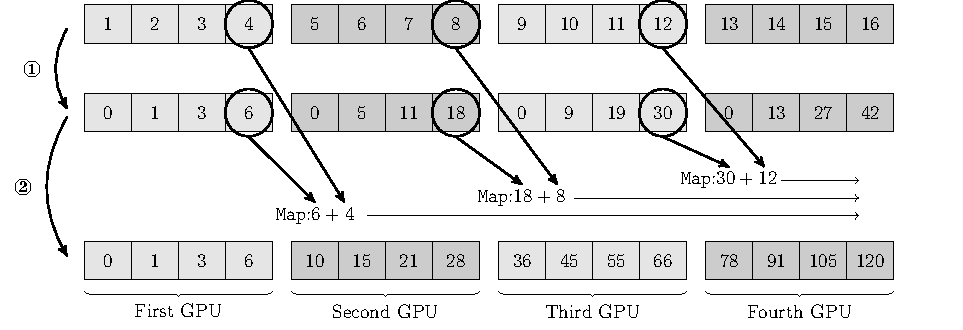
\includegraphics[width=.9\textwidth]{ASHES/scan}
    \caption[Implementation of the \scan skeleton.]%
            {Implementation of the \scan skeleton visualized for four GPUs:
            (1) All GPUs scan their parts independently.
            (2) \map skeletons are created automatically and
             executed to produce the result.}
    \label{fig:scan:impl}
\end{figure*}

%The \SkelCL implementation of the \scan skeleton assumes the \GPUs to have a fixed order, such that each \GPU (except the first one) has a predecessor:
%\begin{enumerate}
% \item Every \GPU executes a local scan algorithm for its local part of data;
% \item The results of all \GPUs are downloaded to the \CPU;
% \item For each \GPU (except the first one), a \map skeleton is implicitly created that combines the result of the \GPU's predecessors with all elements of its part using the user-defined operation of the \scan skeleton;
% \item The newly created \map skeletons compute the final results on all \GPUs.
%\end{enumerate}
The output vector is block-distributed among all \GPUs.





\subsubsection{The Stencil Skeleton}
\label{sec:skelcl:stencil}
In stencil applications, the same computation is performed for each element of a container where the computation depends upon neighboring values.
In \autoref{section:skelcl-programming-model} we defined the \stencil skeleton to simplify the development of stencil applications.
The \SkelCL library provides two implementations of the \stencil skeleton.
The first one, called \code{MapOverlap}, supports simple stencil computations;
the second one, called \code{Stencil}, provides support for more complex stencil computations possibly executed iteratively.
In order to achieve high performance, both implementations \code{MapOverlap} and \code{Stencil} use the \GPU's fast local memory.
Both implementations perform the same basic steps on the \GPU:
first, the data is loaded from the global memory into the local memory;
then, the customizing function is called for every data element by passing a pointer to the element's location in the local memory;
finally, the result of the customizing function is copied back into the global memory.
Although both implementations perform the same basic steps, different strategies are implemented for loading the data from the global into the local memory.

In this subsection, we will start by discussing the \code{MapOverlap} implementation and then discuss the \code{Stencil} implementation.
Finally, we will discuss the implementation of the \stencil skeleton for multi-device systems.

\paragraph{The MapOverlap implementation}

We will use the Gaussian blur as an example application to discuss the \code{MapOverlap} implementation.
The Gaussian blur is a standard image processing algorithm used, among other things, for noise reduction.
The color of every pixel of an image is modified by computing a weighted average of the neighboring pixel color values.
The application will be discussed in more detail in \autoref{sec:gauss}.

\autoref{lst:mapoverlap} shows how the \code{MapOverlap} skeleton implementation is used to express the Gaussian blur.
The \code{mapOverlap} function in \autoref{lst:mapoverlap:factory} is customized with a lambda expression which uses its argument, a \code{Neighborhood} object (\autoref{lst:mapoverlap:neighborhood}), to access the neighboring elements with relative indices (\autoref{lst:mapoverlap:indices1} and \autoref{lst:mapoverlap:indices2}).
The second and third argument of the factory function define the range of the stencil shape and the border handling method (\autoref{lst:mapoverlap:borderHandling}).
The actual computation of the Gaussian blur is omitted from \autoref{lst:mapoverlap} for brevity reasons.

\begin{lstlisting}[%
caption={[Implementation of Gaussian blur using the \stencil skeleton.]%
         Implementation of Gaussian blur using the \code{MapOverlap} implementaion of the \stencil skeleton.},%
float={tb},
label={lst:mapoverlap}]
auto gauss = mapOverlap($\label{lst:mapoverlap:factory}$
  [](Neighborhood<char>& in_img) {$\label{lst:mapoverlap:neighborhood}$
      char ul = in_img[{-1, -1}];$\label{lst:mapoverlap:indices1}$
      ...
      char lr = in_img[{+1, +1}];$\label{lst:mapoverlap:indices2}$
      return computeGaussianBlur(ul, ..., lr); },
  1, BorderHandling::NEUTRAL(0));$\label{lst:mapoverlap:borderHandling}$
\end{lstlisting}


\begin{lstlisting}[%
caption={OpenCL kernel created by the \code{MapOverlap} implementation for the Gaussian blur application.},%
float={tb},
label={lst:mapoverlap:impl}]
#define RANGE (1)   #define NEUTRAL (0)
struct {$\label{lst:mapoverlap:impl:struct:start}$
  local char* data; int row; int col; } char_neighborhood_t;$\label{lst:mapoverlap:impl:struct:end}$

char get(char_neighborhood_t* m, int x, int y) {$\label{lst:mapoverlap:impl:get:start}$
  return m->data[/*computed from RANGE, row, col, x, y*/]; }$\label{lst:mapoverlap:impl:get:end}$

char USER_FUNC(char_neighborhood_t* in_img) {
  char ul = get(in_img, -1, -1);
  ...
  char lr = get(in_img, +1, +1);
  return computeGaussianBlur(ul, ..., lr); }

kernel void mapoverlap(global char* in, global char* out,$\label{lst:mapoverlap:impl:kernel:start}$
          local char* buffer, int numCols, int numRows) {
  ... // load part of in into local buffer$\label{lst:mapoverlap:impl:copy}$
  char_neighborhood_t M;   M.data = buffer;
  M.row = get_local_id(1); M.col = get_local_id(0);
  barrier(CLK_LOCAL_MEM_FENCE);$\label{lst:mapoverlap:impl:barrier}$
  if (/* not out of bound */)
    out[index] = USER_FUNC(&M); }$\label{lst:mapoverlap:impl:call}$
\end{lstlisting}

\autoref{lst:mapoverlap:impl} shows a sketch of the \OpenCL kernel created by the \code{MapOverlap} implementation.
To represent the \code{Neighborhood} object in \OpenCL, a C \code{struct} is created (\autoref{lst:mapoverlap:impl:struct:start}---\autoref{lst:mapoverlap:impl:struct:end}).
A helper function \code{get} (\autoref{lst:mapoverlap:impl:get:start}---\autoref{lst:mapoverlap:impl:get:end}) is created which handles the read access to the data hold by the neighborhood object.
The kernel function \code{mapoverlap}, defined in \autoref{lst:mapoverlap:impl:kernel:start}, first loads the data required by a work-group into a local buffer stored in the fast local \GPU memory (\autoref{lst:mapoverlap:impl:copy}).
It then prepares a neighborhood object and passes it to the customizing function after a boundary check was performed.
A barrier (\autoref{lst:mapoverlap:impl:barrier}) ensures that the loading into the fast local memory has been completed before any work-item executes the customizing function.

Loading of the data into the fast local memory is lengthy and involves performing the boundary checks, therefore, it is not shown in \autoref{lst:mapoverlap:impl}.
%
\begin{figure}
  \begin{centering}
    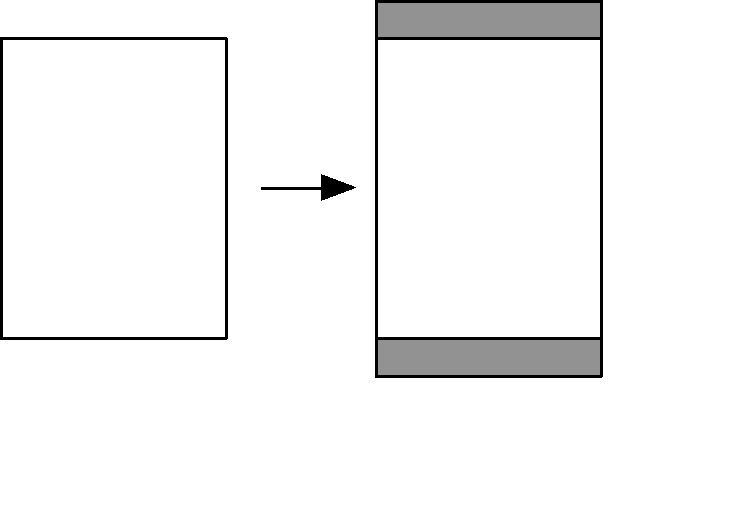
\includegraphics[width=.29\textwidth]{HiStencils/map_overlap}
    \caption[The \code{MapOverlap} implementation of the \stencil skeleton]{The \code{MapOverlap} implementation of the \stencil skeleton prepares a matrix by copying data on the top and bottom}
    \label{fig:mapoverlap:preparation}
    \vspace{-.5em}
  \end{centering}
\end{figure}
%
To minimize the overhead on the \GPU, the \code{MapOverlap} implementation prepares the input matrix on the \CPU before uploading it to the \GPU:
padding elements are appended; they are used to avoid out-of-bounds memory accesses to the top and bottom of the input matrix, as shown in \autoref{fig:mapoverlap:preparation}.
This slightly enlarges the input matrix, but it reduces branching on the \GPU due to avoiding some out-of-bound checks.
In \SkelCL a matrix is stored row-wise in memory on the \CPU and \GPU, therefore, it would be complex and costly to add padding elements on the left and right of the matrix.
To avoid out-of-bound accesses for these regions, the boundary checks are performed on the \GPU.

\paragraph{The Stencil implementation}

We use an iterative stencil application simulating heat flow to discuss the \code{Stencil} implementation.
The application simulates heat spreading from one location and flowing throughout a two-dimensional simulation space.
Let us assume that the heat flows from left to right as indicated by the arrows in \autoref{fig:stencil:first:shape}.
The heat value of a cell is updated based on its (left) neighboring cells.
Multiple iteration steps are required to simulate the flow of heat over a longer distance.

\begin{figure}[t]
  \begin{minipage}[b]{.55\textwidth}
    \begin{lstlisting}[%
      caption={Heat simulation implemented using the \stencil skeleton},%
      label={lst:stencil:first}]
auto heatSim = skelcl::stencil(
 [](Neighborhood<char>& in) {$\label{lst:stencil:first:func:start}$
  char lt = in[{-1, -1}];
  char lm = in[{-1,  0}];
  char lb = in[{-1, +1}];
  return computeHeat(lt,lm,lb);},$\label{lst:stencil:first:func:end}$
 StencilShape(1, 0, 1, 1),$\label{lst:stencil:first:shape}$
 BorderHandling::NEUTRAL(255));$\label{lst:stencil:first:border}$
heatSim(100_iterations,$\label{lst:stencil:first:iterations}$
        simulationSpace);
    \end{lstlisting}
  \end{minipage}%
  \hfill%\hspace{.05\textwidth}
  \begin{minipage}[b]{.38\textwidth}
    \centering
    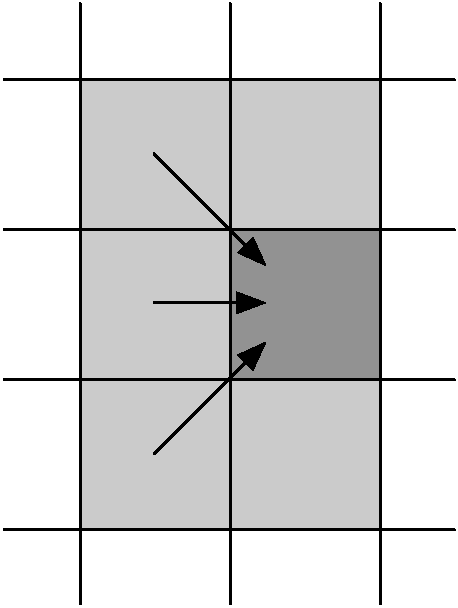
\includegraphics[width=.65\textwidth]{Figures/HiStencils/heat_transfer}
    \caption{Stencil shape for heat simulation}
    \label{fig:stencil:first:shape}
  \end{minipage}
\end{figure}

\autoref{lst:stencil:first} shows the implementation of an iterative stencil application simulating heat transfer in \SkelCL.
The application developer specifies the customizing function (\autoref{lst:stencil:first:func:start}---\autoref{lst:stencil:first:func:end}), as well as the extents of the stencil shape (\autoref{lst:stencil:first:shape}) and the out-of-bound handling (\autoref{lst:stencil:first:border}).
The \code{Stencil} implementation allows the stencil shape's extents to be specified using four values for each of the directions:
up, right, down, and left.
In the example in \autoref{lst:stencil:first}, the heat flows from left to right, therefore, no accesses to the elements to the right are necessary and the stencil space's extents are specified accordingly (note the $0$ in \autoref{lst:stencil:first:shape} representing the extent to the right).
\autoref{fig:stencil:first:shape} illustrates this situation: the dark gray element is updated by using the values from the left.
The specified stencil shape's extent is highlighted in light gray.
In our current implementation, the user has to explicitly specify the stencil shape's extents, which is necessary for performing the out-of-bound handling on the GPU.
In future work, the stencil shape could be inferred from the customizing function using source code analysis in many common cases.
This would help to avoid inconsistencies and free the user from specifying this information explicitly.

Stencil applications often perform stencil computations iteratively, like the heat transfer example which performs multiple iteration steps in order to simulate the transfer of heat over time.
The \code{Stencil} implementation supports iterative execution, which is especially challenging to implement on multi-device systems as we will see later.
On execution of the skeleton, the number of iterations to be performed is specified by the user as the first argument (\autoref{lst:stencil:first:iterations}).
This could be extended in the future, so that the user specifies a function to check if a application specific condition is met and stop the iteration.

The \OpenCL kernel created by the \code{Stencil} implementation looks similar to the \code{MapOverlap} implementation presented in \autoref{lst:mapoverlap:impl}.
The \code{Stencil} implementation uses a slightly different strategy than the \code{MapOverlap} implementation in order to enable the usage of different out-of-bound modes and stencil shapes when using several \stencil skeletons in a sequence, which we discuss in the next paragraph.
To understand why the strategy used by the \code{MapOverlap} implementation is not sufficient for stencil sequences let us consider a situation where two stencil computations are performed one after another and the two stencil shapes used are different.
This cannot be implemented efficiently using \code{MapOverlap}'s implementation strategy, as the input matrix is extended on the \CPU as specified by the first stencil shape.
Therefore, data would have to be downloaded to the \CPU between executions and the data layout would have to be changed.
To avoid this problem, the \code{Stencil} implementation does not append padding elements on the \CPU, but rather manages all out-of-bounds accesses on the \GPU, which slightly increases branching in the code, but enables a more flexible usage of the skeleton.


\paragraph{Sequence of Stencil Operations}
Many real-world applications perform different stencil operations in sequence, like the popular \emph{Canny algorithm}~\cite{NixonAg2012} used for detecting edges in images.
For the sake of simplicity, we consider a version which applies the following steps:
1)~a noise reduction operation is applied, e.\,g., a Gaussian blur;
2)~an edge detection operator like the Sobel filter is applied;
3)~the so-called non-maximum suppression is performed, where all pixels in the image are colored black except pixels being a local maximum;
4)~a threshold operation is applied to produce the final result.
A more complex version of the algorithm performs the edge tracking by hysteresis as an additional step.

Using the \SkelCL library, each single step of the Canny algorithm can be expressed using the \stencil skeleton, as shown in \autoref{lst:stencil:canny}.
The threshold operation performed as the last step, does not need access to, neighboring elements, because the user function only checks the value of a single pixel.
The \code{Stencil} implementation automatically uses the implementation of the simpler (and thus faster) \map skeleton when the user specifies a stencil shape whose extents are $0$ in all directions.
The single steps are combined into a single object of type \code{StencilSequence} which can be executed like a \stencil skeleton.
On execution, it passes its input data to the first stencil defined in the sequence, its output to the next stencil, and so forth.

\begin{lstlisting}[%
  caption={Structure of the Canny algorithm implemented by a sequence of skeletons.},%
  float={tb},
  label={lst:stencil:canny}]
auto gauss     = stencil(...);
auto sobel     = stencil(...);
auto nms       = stencil(...);
auto threshold = stencil(...);

StencilSequence<Pixel(Pixel)>
    canny(gauss, sobel, nms, threshold);
\end{lstlisting}

\paragraph{Targeting Multi-\GPU Systems}
The implicit and automatic support of systems with multiple \OpenCL devices is one of the key features of \SkelCL.
By using distributions, \SkelCL completely liberates the user from error-prone and low-level explicit programming of data (re)distributions on multiple \GPUs.

The \code{MapOverlap} implementation uses the overlap distribution with \textit{border regions} in which the elements calculated by a neighboring device are located.
When it comes to iteratively executing a skeleton, data has to be transferred among devices between iteration steps, in order to ensure that data for the next iteration step is up-to-date.
As the \code{MapOverlap} implementation does not explicitly supports iterations, its implementation is not able to exchange data between devices besides a full down- and upload of the matrix.
% In addition, data exchange has to be performed after each iteration.

The \code{Stencil} implementation explicitly supports iterative execution and, therefore, only exchanges elements from the border region and does not perform a full down- and upload of the matrix, as the \code{MapOverlap} implementation does.
\autoref{fig:syncDevices} shows the \textit{device synchronizations}, \ie, the data exchange performed between two iterations by the \code{Stencil} implementation.
Only the appropriate elements in the \emph{inner border region}, \ie, the border regions adjacent to two \OpenCL devices, are downloaded and stored as \texttt{std::vector}s in a \texttt{std::vector}.
Within the outer vector, the inner vectors are swapped pair-wise on the host, so that the inner border regions can be uploaded in order to replace the out-of-date border regions.

\begin{figure}[tb]
  \centering
  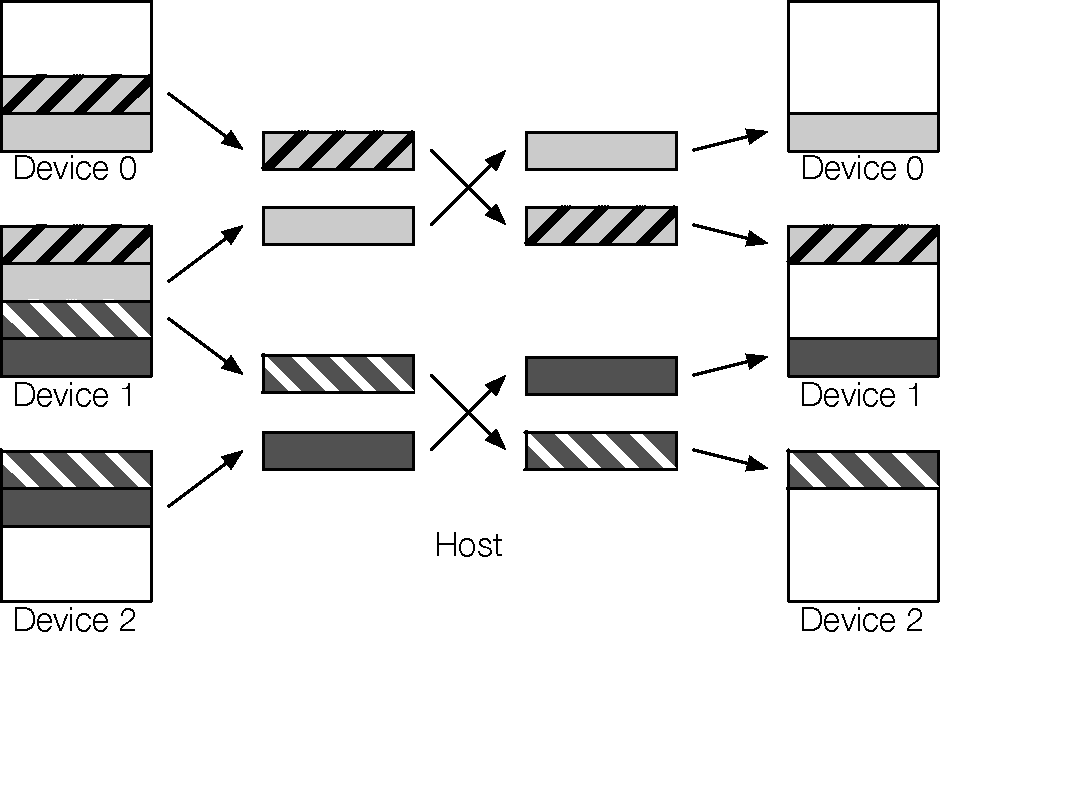
\includegraphics[width=.75\columnwidth]{HiStencils/data_exchange}
  \caption[Device synchronization for three devices during the execution of the \stencil skeleton.]
          {\small Device synchronization for three devices. Equally patterned and colored chunks represent the border regions and their matching inner border region. After the download of the appropriate inner border regions, they are swapped pair-wise on the host. Then the inner border regions are uploaded in order to replace the outdated border regions.}
  \label{fig:syncDevices}
  \vspace{1em}
\end{figure}


By enlarging the number of elements in the border regions, multiple iteration steps can be performed on each device before exchanging data.
However, this introduces redundant computations, such that a trade-off between data exchange and redundant computations has to be found.
For the \code{Stencil} implementation, the user can specify the number of iterations between device synchronizations.
\cite{Breuer2014} discusses the effects of exploring this parameter space.
For the investigated applications, the effect of choosing different numbers of iterations between device synchronization was not very large.


\subsubsection{The \allpairs Skeleton}
The \allpairs skeleton defined in \autoref{section:skelcl-programming-model} applies a customizing function to all pairs of vectors from two matrices.
There exist two version of the skeleton: the generic \allpairs skeleton introduced in \autoref{sec:allpairs_skeleton} and the specialized \allpairs skeleton introduced in \autoref{sec:opt_allpairs_skeleton}.
In the specialized version the customizing function is expressed as a composition of the \zip and \reduce skeleton.

In this subsection, we will first discuss the generic and then the specialized implementation.
We will also estimate the performance benefit gained by the specialized implementation.
Finally, we will discuss the implementation of the \allpairs skeleton on multi-device systems.

\paragraph{The Generic Allpairs Skeleton}
\begin{lstlisting}[%
caption={Matrix multiplication expressed using the generic \allpairs skeleton.},%
float=t,%
numbers=left,%
label={lst:allpairs:generic:impl}]
auto mm = allpairs([](const Vector<float>& a,
                      const Vector<float>& b) {
                        float c = 0.0f;
                        for (int i = 0; i < a.size(); ++i)
                          c += a[i] * b[i];
                        return c; });
\end{lstlisting}

\autoref{lst:allpairs:generic:impl} shows the program for computing matrix multiplication using the generic \allpairs skeleton.
The implementation of the customizing function is straightforward.
It is expressed as a lambda expression that receives a pair of vectors, multiplies their elements and sums them up.

\autoref{lst:allpairs:generic:kernel} shows the \OpenCL kernel created after adding and adapting the generic allpairs implementation.
The customizing function (\autoref{lst:allpairs:generic:kernel:funcStart}---\autoref{lst:allpairs:generic:kernel:funcEnd}) has been transformed by the \code{skelclc} compiler.
The vector class has been replaced by an \OpenCL representation (defined in \autoref{lst:allpairs:generic:kernel:structStart} and \autoref{lst:allpairs:generic:kernel:structEnd}) and the element access to the vectors has been replaced by computations of the matching indices.
This implementation assumes that the rows of the first matrix are combined with the columns of the second matrix, as it is required for the matrix multiplication.
% The implementation could easily be extended to support different behavior as well.

The \code{allpairs} kernel function prepares instances of the \code{struct} replacing the vector class in \autoref{lst:allpairs:generic:kernel:prepareStart}---\autoref{lst:allpairs:generic:kernel:prepareEnd}.
After performing a boundary check, the customizing function is called in \autoref{lst:allpairs:generic:kernel:call}.
This \OpenCL kernel is executed once for every element of the output matrix $C$.

\begin{lstlisting}[%
caption={OpenCL kernel used in the implementation of the generic \allpairs skeleton.},%
float=t,%
numbers=left,%
label={lst:allpairs:generic:kernel}]
struct {$\label{lst:allpairs:generic:kernel:structStart}$
  global float* data; int size; int index; } float_matrix_t;$\label{lst:allpairs:generic:kernel:structEnd}$

float USER_FUNC(float_matrix_t* a, float_matrix_t* b) {$\label{lst:allpairs:generic:kernel:funcStart}$
   float c = 0.0f;
   for (int i = 0; i < a->size; ++i) {
     c +=   a->data[a->index * a->size + i]
          * b->data[i * b->size + b->index]; }
   return c; }$\label{lst:allpairs:generic:kernel:funcEnd}$

kernel void allpairs(const global float* Ap,
                     const global float* Bp,
                           global float* Cp,
                     int n, int d, int m) {
  int col = get_global_id(0); int row = get_global_id(1);
  float_matrix_t A; A.data = Ap; Am.size = d; A.index = row;$\label{lst:allpairs:generic:kernel:prepareStart}$
  float_matrix_t B; B.data = Bp; Bm.size = m; B.index = col;$\label{lst:allpairs:generic:kernel:prepareEnd}$
  if (row < n && col < m)
    Cp[row * m + col] = USER_FUNC(&A, &B); }$\label{lst:allpairs:generic:kernel:call}$
\end{lstlisting}

This generic implementation makes no assumption about the order in which the customizing function (\texttt{USER\_FUNC}) accesses the elements of its two input vectors.
In this generic case, we cannot assume that the two vectors fit entirely into the fast but restricted GPU local memory.
Therefore, we have to use only the slower global memory in the generic implementation.
On modern GPUs, accesses to the global memory are very expensive, taking up to 800 processor cycles, as compared to only few cycles required to access the local memory~\cite{CUDAProgrammingGuide}.

Let us assume targeting \GPU architectures and estimate the number of global (and, therefore, expensive) memory accesses required for computing an element of the matrix multiplication in the generic case.
One global memory read access for every element of both input vectors is performed, and a single global memory write access is required to write the result into the output matrix.
Therefore,
\begin{equation}
  n\cdot m\cdot (d + d + 1)
  \label{eq:mm:accesses}
\end{equation}
global memory accesses are performed in total, where $n$ and $m$ are the height and width of matrix $C$ and $d$ is the width of $A$ and the height of $B$.
By using the fast but small local memory, this number of global memory accesses can be reduced and, thus, performance can be improved, as we will see in the next paragraph.
Using the local memory for matrix multiplication is a well-known optimization which we systematically apply to a generic skeleton, rather than to a particular application as usually done in the literature.

\paragraph{The Specialized Allpairs Skeleton}
\autoref{lst:allpairs:special:impl} shows matrix multiplication expressed using the specialized \allpairs skeleton.
\begin{lstlisting}[%
caption={Matrix multiplication expressed using the specialized \allpairs skeleton.},%
float=b,%
numbers=left,%
label={lst:allpairs:special:impl}]
auto mult  = zip([](float x, float y){return x*y;});
auto sumUp = reduce([](float x, float y){return x+y;}, 0);
auto mm    = allpairs(sumUp, mult);
\end{lstlisting}
%
By expressing the customizing function of the \allpairs skeleton as a \zip-\reduce composition, we provide to the skeleton implementation additional semantic information about the memory access pattern of the customizing function, thus allowing for improving the performance.
Our idea of optimization is based on the \OpenCL programming model that organizes \emph{work-items} (i.\,e., threads executing a kernel) in \emph{work-groups} which share the same \GPU local memory.
By loading data needed by multiple work-items of the same work-group into the local memory, we can avoid repetitive accesses to the global memory.

\begin{figure}[b]
  \centering
  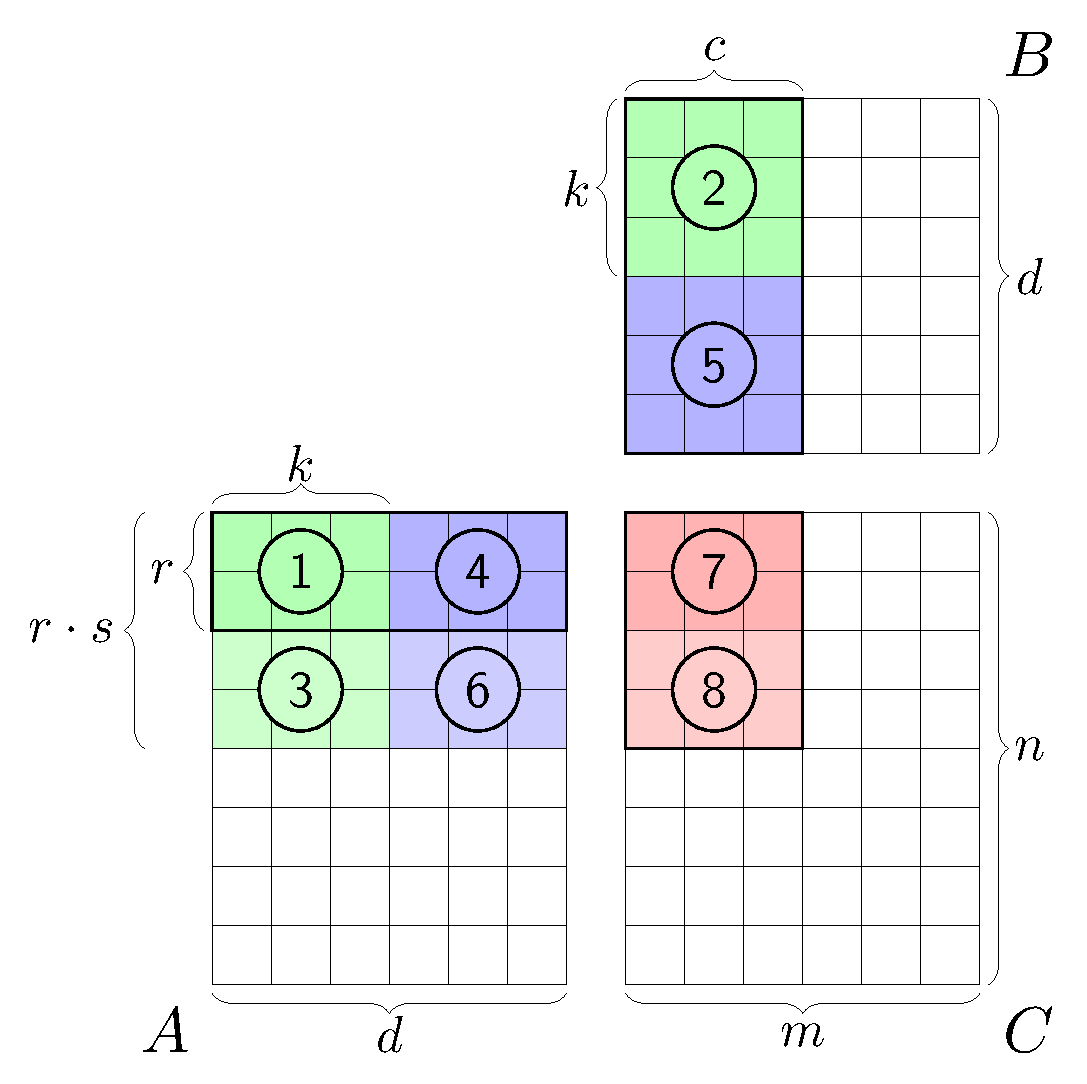
\includegraphics[width=.4\textwidth]{HLPP/memory_access}
  \caption{Implementation schema of the specialized \allpairs skeleton.}
  \label{fig:memory_access}
\end{figure}
For the \allpairs skeleton with the \zip-\reduce customizing function, we can adopt the implementation schema for \GPUs from~\cite{SarjeAl2013}, as shown in \autoref{fig:memory_access}.
We allocate two arrays in the local memory, one of size $r\times k$ ($r=2$, $k=3$ in \autoref{fig:memory_access}) for elements of $A$ and one of size $k\times c$ ($c=3$ in \autoref{fig:memory_access}) for elements of $B$.
A work-group consisting of $c\times r$ work-items computes $s$ blocks ($s=2$ in \autoref{fig:memory_access}) of the result matrix $C$.
In \autoref{fig:memory_access}, the two blocks marked as \circled{7} and \circled{8} are computed by the same work-group as follows.
In the first iteration, the elements of blocks \circled{1} and \circled{2} are loaded into the local memory and combined following the \zip-\reduce pattern.
The obtained intermediate result is stored in block \circled{7}.
Then, the elements of block \circled{3} are loaded and combined with the elements from \circled{2} which still reside in the local memory.
The intermediate result is stored in block \circled{8}.
In the second iteration, the algorithm continues in the same manner with blocks \circled{4}, \circled{5}, and \circled{6}, but this time, the elements of the blocks are also combined with the intermediate results of the first iteration, which are stored in blocks \circled{7} and \circled{8}.
The advantage of computing multiple blocks by the same work-group is that we keep the elements of $B$ in the local memory when computing the intermediate results, \ie, we do not reload block \circled{2} twice for the computation of blocks \circled{7} and \circled{8}.

Every element loaded from the global memory is used by multiple work-items:
\eg, the upper left element of block \circled{1} is loaded only once from the global memory, but used three times:
in the computation of the upper left, upper middle, and upper right elements of \circled{7}.
In general, every element loaded from $A$ is reused $c$ times, and every element from $B$ is reused $r\cdot s$ times.
As the intermediate results are stored in the global memory of matrix $C$, we perform two additional memory accesses (read/write) for every iteration, \ie, $2\cdot \frac{d}{k}$ in total.
Therefore, instead of $n\cdot m\cdot (d + d + 1)$ (see \autoref{eq:mm:accesses}) global memory accesses necessary when using the non-specialized skeleton only
\begin{equation}
  n\cdot m\cdot (\frac{d}{r\cdot s} + \frac{d}{c} + 2\cdot \frac{d}{k})
\end{equation}
global memory accesses are performed.
By increasing the parameters $s$ and $k$, or the number of work-items in a work-group ($c$ and $r$), more global memory accesses can be saved.
However, the work-group size is limited by the \GPU hardware.
While the parameters can be chosen independently of the matrix sizes, we have to consider the amount of available local memory.
\cite{Friese2013}~and~\cite{SarjeAl2013}~discuss how suitable parameters can be found by performing runtime experiments.
In~\cite{Friese2013} the parameters $c = 32$, $r=8$, $s=32$, and $k=64$ are used on modern \GPU hardware showing good performance.

We will report measurements of the performance difference for the two skeleton implementations on real hardware in \autoref{chapter:skelcl-evaluation}.

\paragraph{The Allpairs Skeleton using Multiple GPUs}
\label{sec:allpairs:multi_gpu}
\begin{figure}[b]
  \centering
  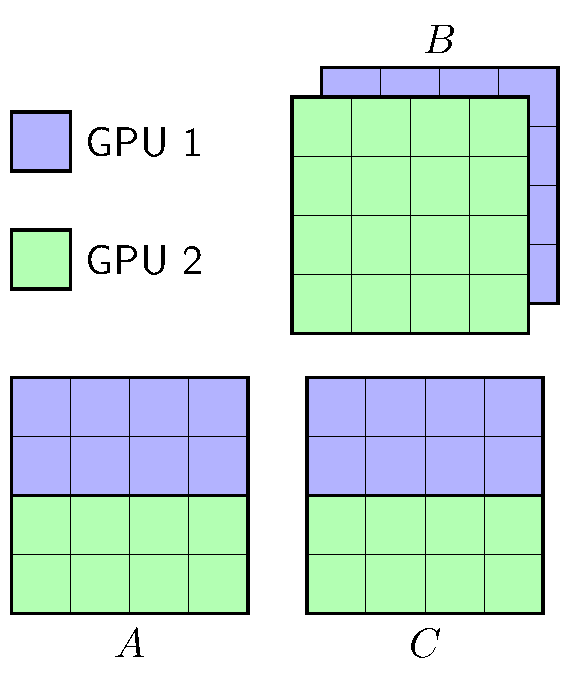
\includegraphics[width=.3\textwidth]{HLPP/multi_gpu}
  \caption[Data distributions used for the \allpairs skeleton for a system with two \GPUs.]%
          {Data distributions used for a system with two \GPUs: matrices $A$ and $C$ are \emph{block} distributed, matrix $B$ is \emph{copy} distributed.}
  \label{fig:multi_gpu}
\end{figure}

The \allpairs skeleton can be efficiently implemented not only on systems with a single \GPU, but on multi-\GPU systems as well.
The necessary data distribution can be easily expressed using two of \SkelCL's \emph{distributions}, as shown in \autoref{fig:multi_gpu}:
Matrix $B$ is \emph{copy} distributed, \ie, it is copied entirely to all \GPUs in the system.
Matrix $A$ and $C$ are \emph{block} distributed, \ie, they are row-divided into as many equally-sized blocks as \GPUs are available;
each block is copied to its corresponding \GPU.
Following these distributions, each \GPU computes one block of the result matrix $C$.
In the example with two GPUs shown in \autoref{fig:multi_gpu}, the first two rows of $C$ are computed by \GPU 1 and the last two rows by \GPU 2.
The \allpairs skeleton automatically selects these distributions, therefore, the same source code can be used when using a single \GPU or multiple \GPUs.











\subsection{Memory Management Implementation}
\label{section:skelcl-library:memory-management}
In the \SkelCL programming model, the user managed memory using \emph{container data types}.
In the \SkelCL library, the two container data types -- vector and matrix -- are implemented as template classes.
This generic implementation allows for storing data items of any primitive C/\Cpp data type (\eg, \code{int}), as well as user-defined data structures (\code{struct}s).
The implementations follow the \emph{resource acquisition is initialization} (RAII) idiom, which means that they automatically allocate needed resources and free them automatically when the lifetime of the container ends.

\paragraph{The SkelCL Vector}
The \SkelCL vector replicates the interface of the vector from the \Cpp Standard Template Library (\STL), \ie, it can be used as a drop-in replacement of the standard vector.
Internally, a vector comprises pointers to the corresponding areas of main memory (accessible by the host) and device memory.
The vector holds one pointer for the host and one pointer for each device available.
Memory on the devices is allocated automatically, according to the distribution of the vector:
while for a single distributed vector only memory on a single device is allocated, for a vector distributed with the copy, block, or overlap distribution memory on all devices is allocated.
The selected distribution obviously also influences how big the buffers allocated on the devices will be.

Before the execution of a skeleton, the input vector's implementation ensures that all of its data is available on the devices.
This might result in implicit data transfers from the host memory to device memory.
The data of the output vector is not copied back to the host memory but rather resides in the device memory.
Before every data transfer, the vector implementation checks whether the data transfer is necessary;
only then the data is actually transferred.
Hence, if an output vector is used as the input to another skeleton, no further data transfer is performed.
This \emph{lazy copying} in \SkelCL defers data transfers as long as possible or avoids them completely and, thus, minimizes the costly data transfers between host and device.
While all data transfers are performed implicitly by \SkelCL, we understand that advanced application developers may want to have a fine-grained control over the data transfers between host and devices.
For that purpose, \SkelCL offers a set of \APIs which developers can use to explicitly initiate and control the data transfer to and from the devices.

% Implementing such data transfers in \OpenCL manually is a cumbersome task:
% data has to be downloaded to the host before it can be uploaded to other devices, including the corresponding length and offset calculations;
% this results in a lot of low-level code which is completely hidden when using \SkelCL.


\paragraph{The SkelCL Matrix}
The \SkelCL matrix offers an easy to use interface similar to the interface of the vector.
Data is stored in the row-major order and iterators are provided to iterate first over rows and then inside of a single row to access a particular element.
For the copy, block, and overlap distributions, the matrix is divided across rows.
A single row is never split across multiple devices, which simplifies the memory management.
Besides offering an interface to access elements on the host, the matrix also offers an interface for accessing elements on the device by using two-dimensional indices.
This frees the application developer from performing cumbersome index calculations manually.










\subsection{Data Distribution Implementation}
\label{section:skelcl-library:distribution}
The data distributions determine how the data of a container is distributed across multiple devices.
In the \SkelCL library implementation, there exists a class for each data distribution encapsulating the behavior of the distribution.
Every container stores its current data distribution as a member variable.
When the data of the container has to be transferred to or from the devices, the data distribution object is invoked to perform the data transfer operation.

% The data distribution of a container can be changed at runtime either explicitly by the programmer or implicitly by the \SkelCL implementation.
% A change of distribution implies data exchanges between multiple devices and the host, which are performed implicitly by \SkelCL.
% These implicit data exchanges are also performed lazily, \ie, only if really necessary, as described in the previous subsection.

% A special situation arises when the distribution is changed from the \emph{copy} distribution, where each device holds its own full copy of the data.
% In such a case, each device may hold a different version of the container as data modifications are only performed locally on the device.
% In order to maintain \SkelCL's concept of a self-contained container, these different versions must be combined using a user-specified function when the distribution is changed.
% If no function is specified, the copy of the first device is taken as the new version of the container; the copies of the other devices are discarded.

